\section{Results Analysis - Parabolic Model}

So how does the parabolic model perform? We'll take a look at 2 test cases. In the first case the parabolic model will appear adequate, but in the second we'll see it's not quite good enough.

\subsection{Test Case: Low Drag}

%% Test 1

\begin{figure}[t]
\centering
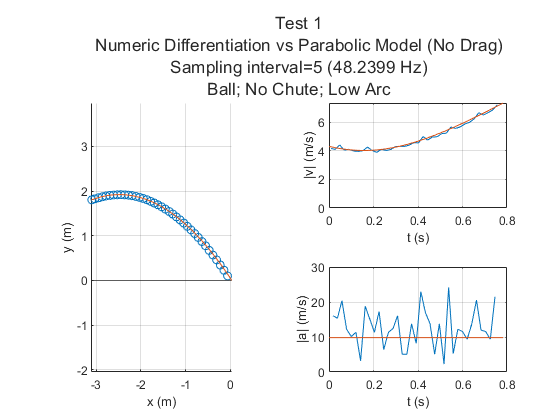
\includegraphics[width=0.9\linewidth]{images/Analysis1_Test1_Fig5_NoDrag.png}
\caption{\label{fig:Analysis1_Test1_Fig5_NoDrag} Fitting the parabolic model to sampled position data for a ball with no parachute. Left: Sampled position (blue) with the fit trajectory (orange). Right: Velocity and acceleration computed using numeric differentiation (blue) and the model's velocity and acceleration (orange). For low-drag scenarios, the parabolic model appears adequate.}
\end{figure}

We started by fitting our parabolic model on some data of just the plain ball with no parachute attached. It was thrown in a low arc; keeping the speed low and minimizing drag effects. This should be the best-case scenario for the parabolic model. The data is shown in Fig.~\ref{fig:Analysis1_Test1_Fig5_NoDrag}. 

At first glance, this model is actually looking pretty decent. There aren't any huge problems with the trajectory plot at this scale. Looking at the numeric differentiation, it's clear that there's plenty of noise in the signal. The velocity plot has some noise, and the model's velocity forms a smooth line through the middle of it. The noise in the signal makes the numeric differentiation's acceleration data nearly useless, but the model's acceleration is a constant 1g as expected. 

This is all good news because it verifies that the code we've been working on up until now works as intended. There certainly was no need for multiple cycles of struggle and debugging.\footnote{This is sarcasm.} In addition to verifying the code, if this projectile had been the only design we cared about, we would probably just call it a day here and save ourselves a lot of work by not implementing the linear drag model. Alas, someone had the bright idea to put a parachute on that ball. Let's look at that data next.


\subsection{Test Case: High Drag}

%% Test 4

\begin{figure}[t]
\centering
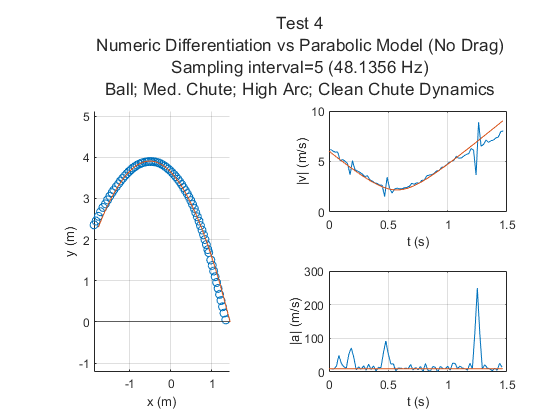
\includegraphics[width=0.9\linewidth]{images/Analysis1_Test4_Fig5_NoDrag.png}
\caption{\label{fig:Analysis1_Test4_Fig5_NoDrag} Fitting the parabolic model to sampled position data for a ball with a parachute. Judging by the position plot, the parabolic model is unable to adequately capture the motion of this system.}
\end{figure}

\begin{figure}[t]
\centering
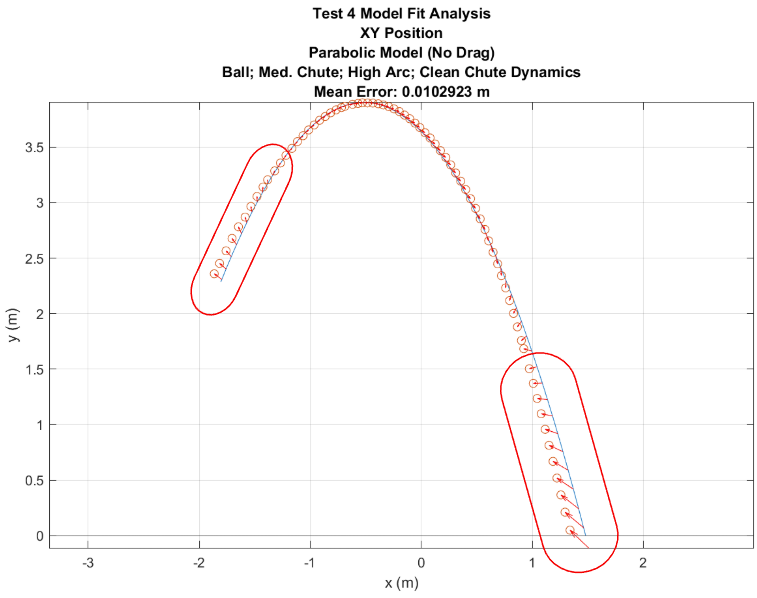
\includegraphics[width=0.9\linewidth]{images/Analysis1_Test4_Err_NoDrag.png}
\caption{\label{fig:Analysis1_Test4_Err_NoDrag} A closer look at the failure of the parabolic model. Red vectors show the error for each sampled position. The highlighted regions at the start and end of the trajectory show how the parabolic model deviates from the observed data.}
\end{figure}

Here the limitations of the parabolic model become more apparent. The data for a higher drag scenario is shown in Fig.~\ref{fig:Analysis1_Test4_Fig5_NoDrag}, and Fig.~\ref{fig:Analysis1_Test4_Err_NoDrag} presents the trajectory in more detail. The model fits decently around the apex, but is way off at the start and end. Clearly, drag plays a more significant role than the parabolic model can account for. 

At this point it's tempting to see the model failing in this way and immediately take this as the justification we need to invest in the linear drag model. But let's do a quick vibe check. What if we didn't expect it to fail like this? Does it make sense that incorporating linear drag would help? After all, it isn't just the drag we increased. Attaching the chute via strings turns this into a complex multibody system. What trajectory would we expect from two point masses attached by spring? Answering these questions is left as an exercise for the reader. We will carry on with the analysis assuming linear drag will be the solution.


\subsection{Test Case: High Drag - Frame by Frame}

\begin{figure*}[t!]
    \centering
    \begin{subfigure}[t]{0.5\textwidth}
        \centering
        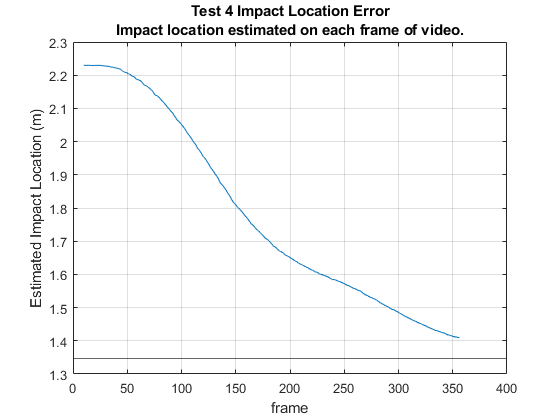
\includegraphics[width=\textwidth]{images/Analysis1_Test4_ImpLocPlot_NoDrag.png}
        \caption{}
    \end{subfigure}%
    ~ 
    \begin{subfigure}[t]{0.5\textwidth}
        \centering
        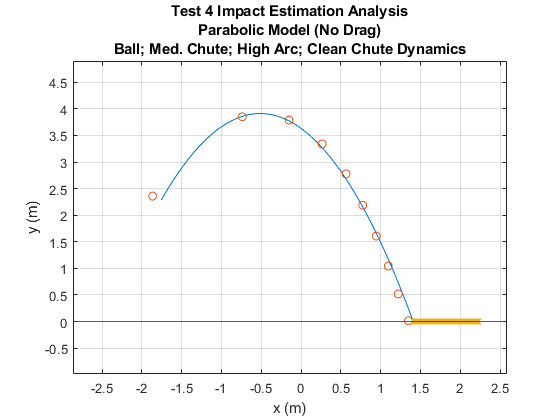
\includegraphics[width=\textwidth]{images/Analysis1_Test4_ImpLocHist_NoDrag.png}
        \caption{}
    \end{subfigure}
    \caption{\label{fig:Test4_NoDrag_FrameByFrame} Frame-by-frame impact location estimation for a ball with a parachute using the parabolic model. (a) Impact location over time. (b) Impact locations marked.}
\end{figure*}

We now consider a form of analysis where we fit a trajectory model to the sampled data frame-by-frame; as sort of an analog to using this tool in real-time. For each frame of video data, we select 10 points spaced between the start of the data up until the current frame. We then fit a trajectory to that subset of the data and record the predicted impact location. This is done for each frame of the video. Results are shown in Fig.~\ref{fig:Test4_NoDrag_FrameByFrame}. 

What becomes immediately apparent is that the estimates derived frame-by-frame failed to align with the observed impact position. Even up to the moment of impact. And it's not just noise, there's clearly some unmodeled behavior causing this offset in the error. There's one clear conclusion that we draw from this: The parabolic model, which completely ignores drag, is simply inadequate for predicting the trajectory when drag is significant. 

